\newpage

\section*{ $^{44}$Ca(n,$\gamma$)$^{45}$Ca }

Power Level: 100 kW(th) \\
Time at Power: 60.0 m \\
Wait Time:  2.0 d \\
Counting Time: 60.0 m \\
Total Activity at Removal: 9.68e-04 $\mu Ci$

\begin{table*}[h]
\centering
\begin{tabular}{ |c|c|c|c|c|c| }
 \hline
 Position & Mass $mg$ & Counting Activity $\mu Ci$ & Area (Counts) & Error \% \\
 \hline 
 1 & 0.23 & 2.01e-04 & 7.24e-16 & 3715384198.7422 \\ 
\hline
 2 & 0.23 & 3.07e-04 & 1.11e-15 & 3001496596.0805 \\ 
\hline
 3 & 0.23 & 2.85e-04 & 1.03e-15 & 3116189888.2917 \\ 
\hline
 4 & 0.23 & 1.67e-04 & 6.04e-16 & 4070494343.0619 \\ 
\hline
\end{tabular}
\end{table*}

\begin{figure}[h]
\centering
\begin{subfigure}{.5\textwidth}
  \centering
     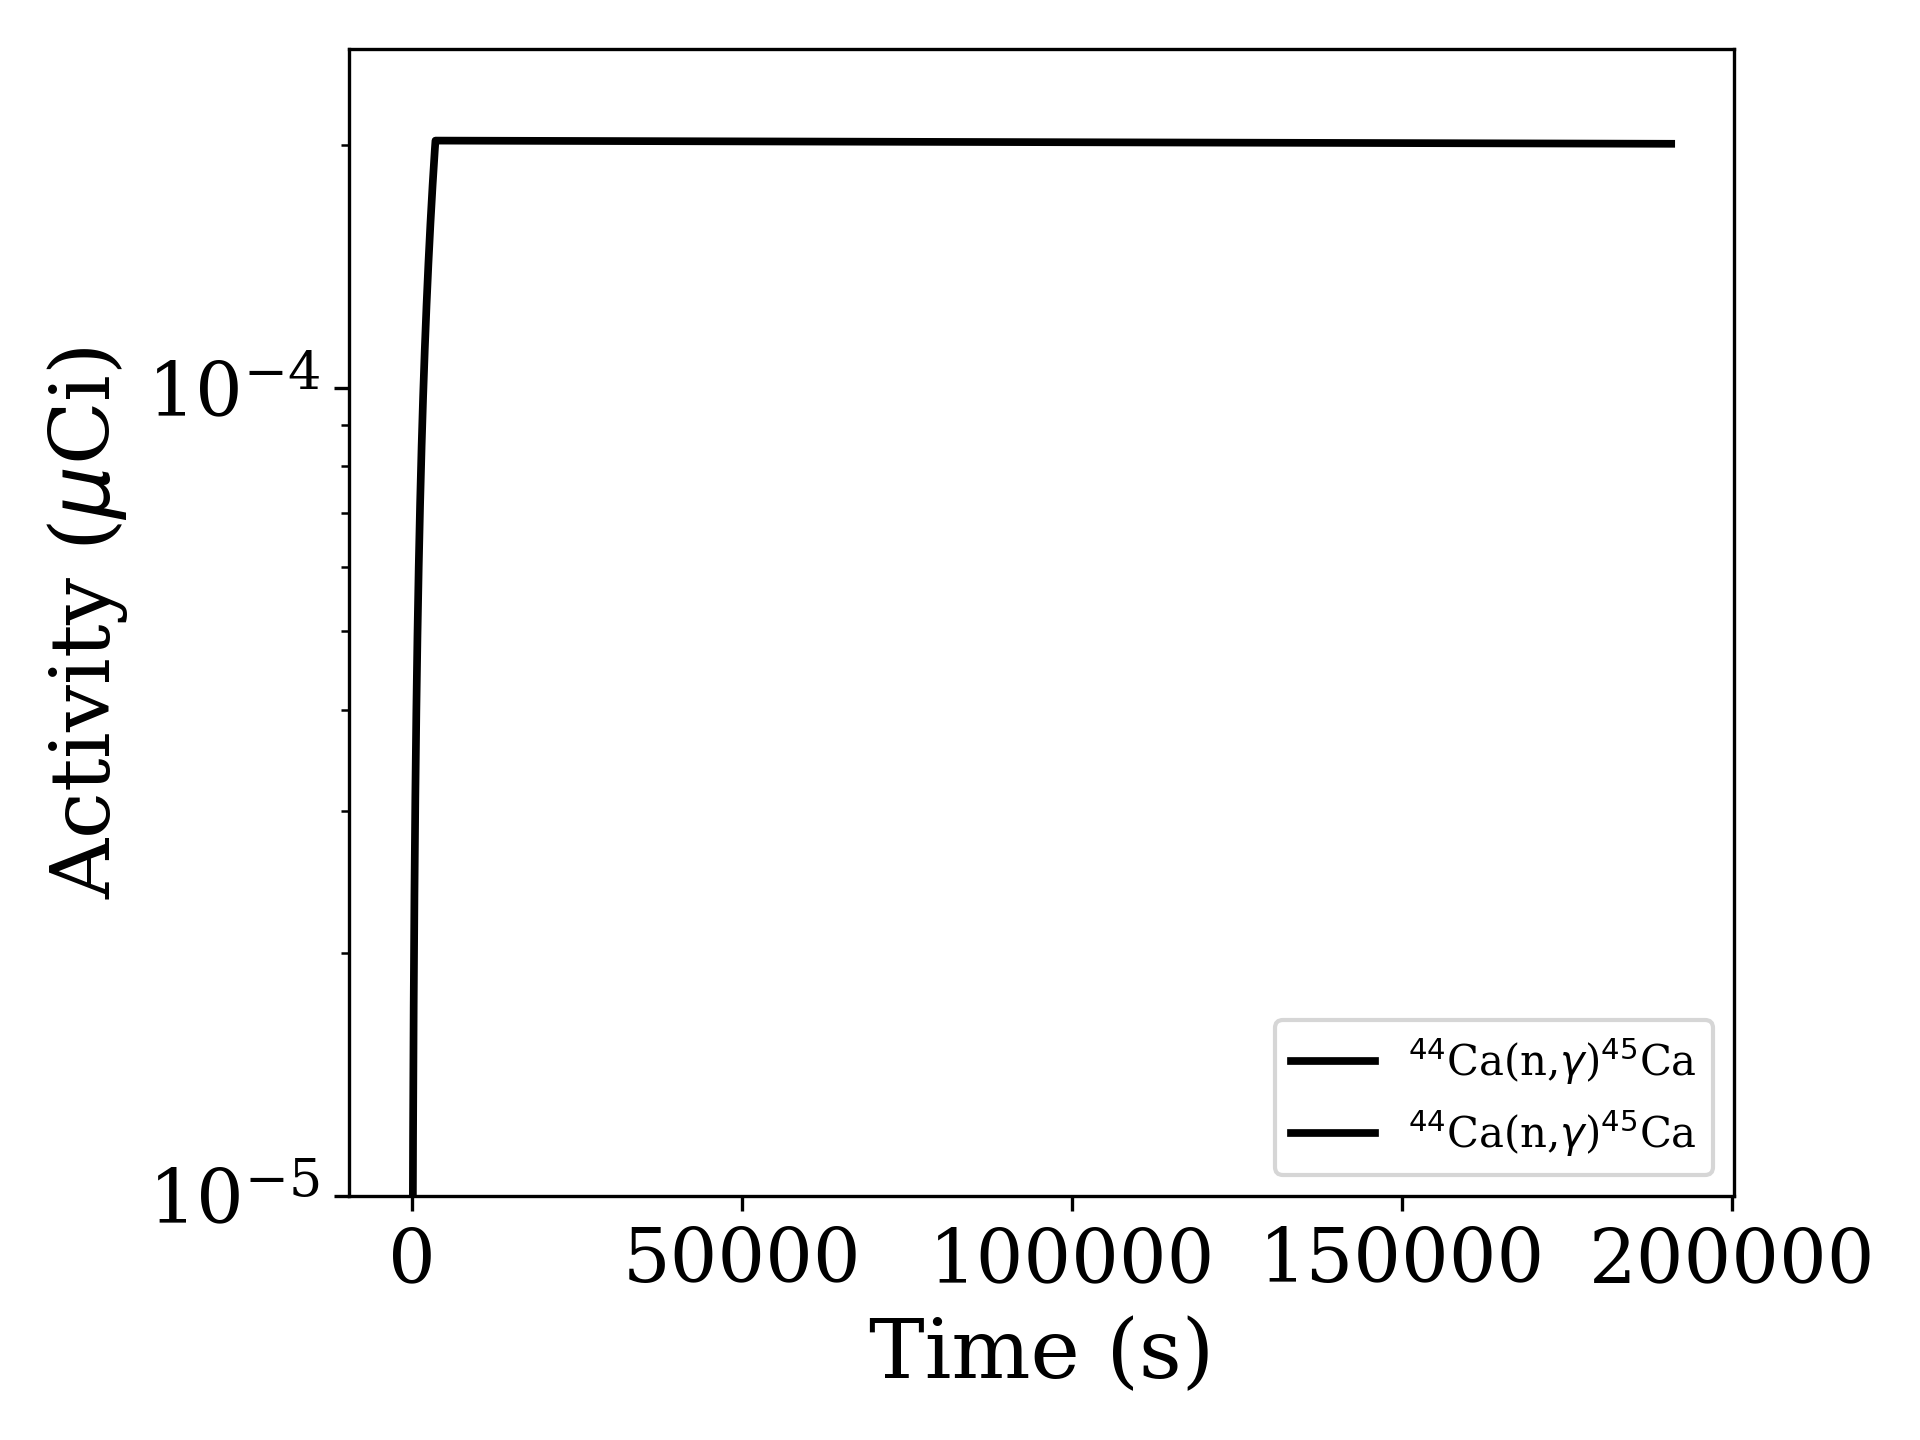
\includegraphics[width=.8\textwidth]{plot/Ca-44(n,gamma)Ca-45_library1} 

  \caption{A subfigure}
  \label{fig:sub1}
\end{subfigure}%
\begin{subfigure}{.5\textwidth}
  \centering
     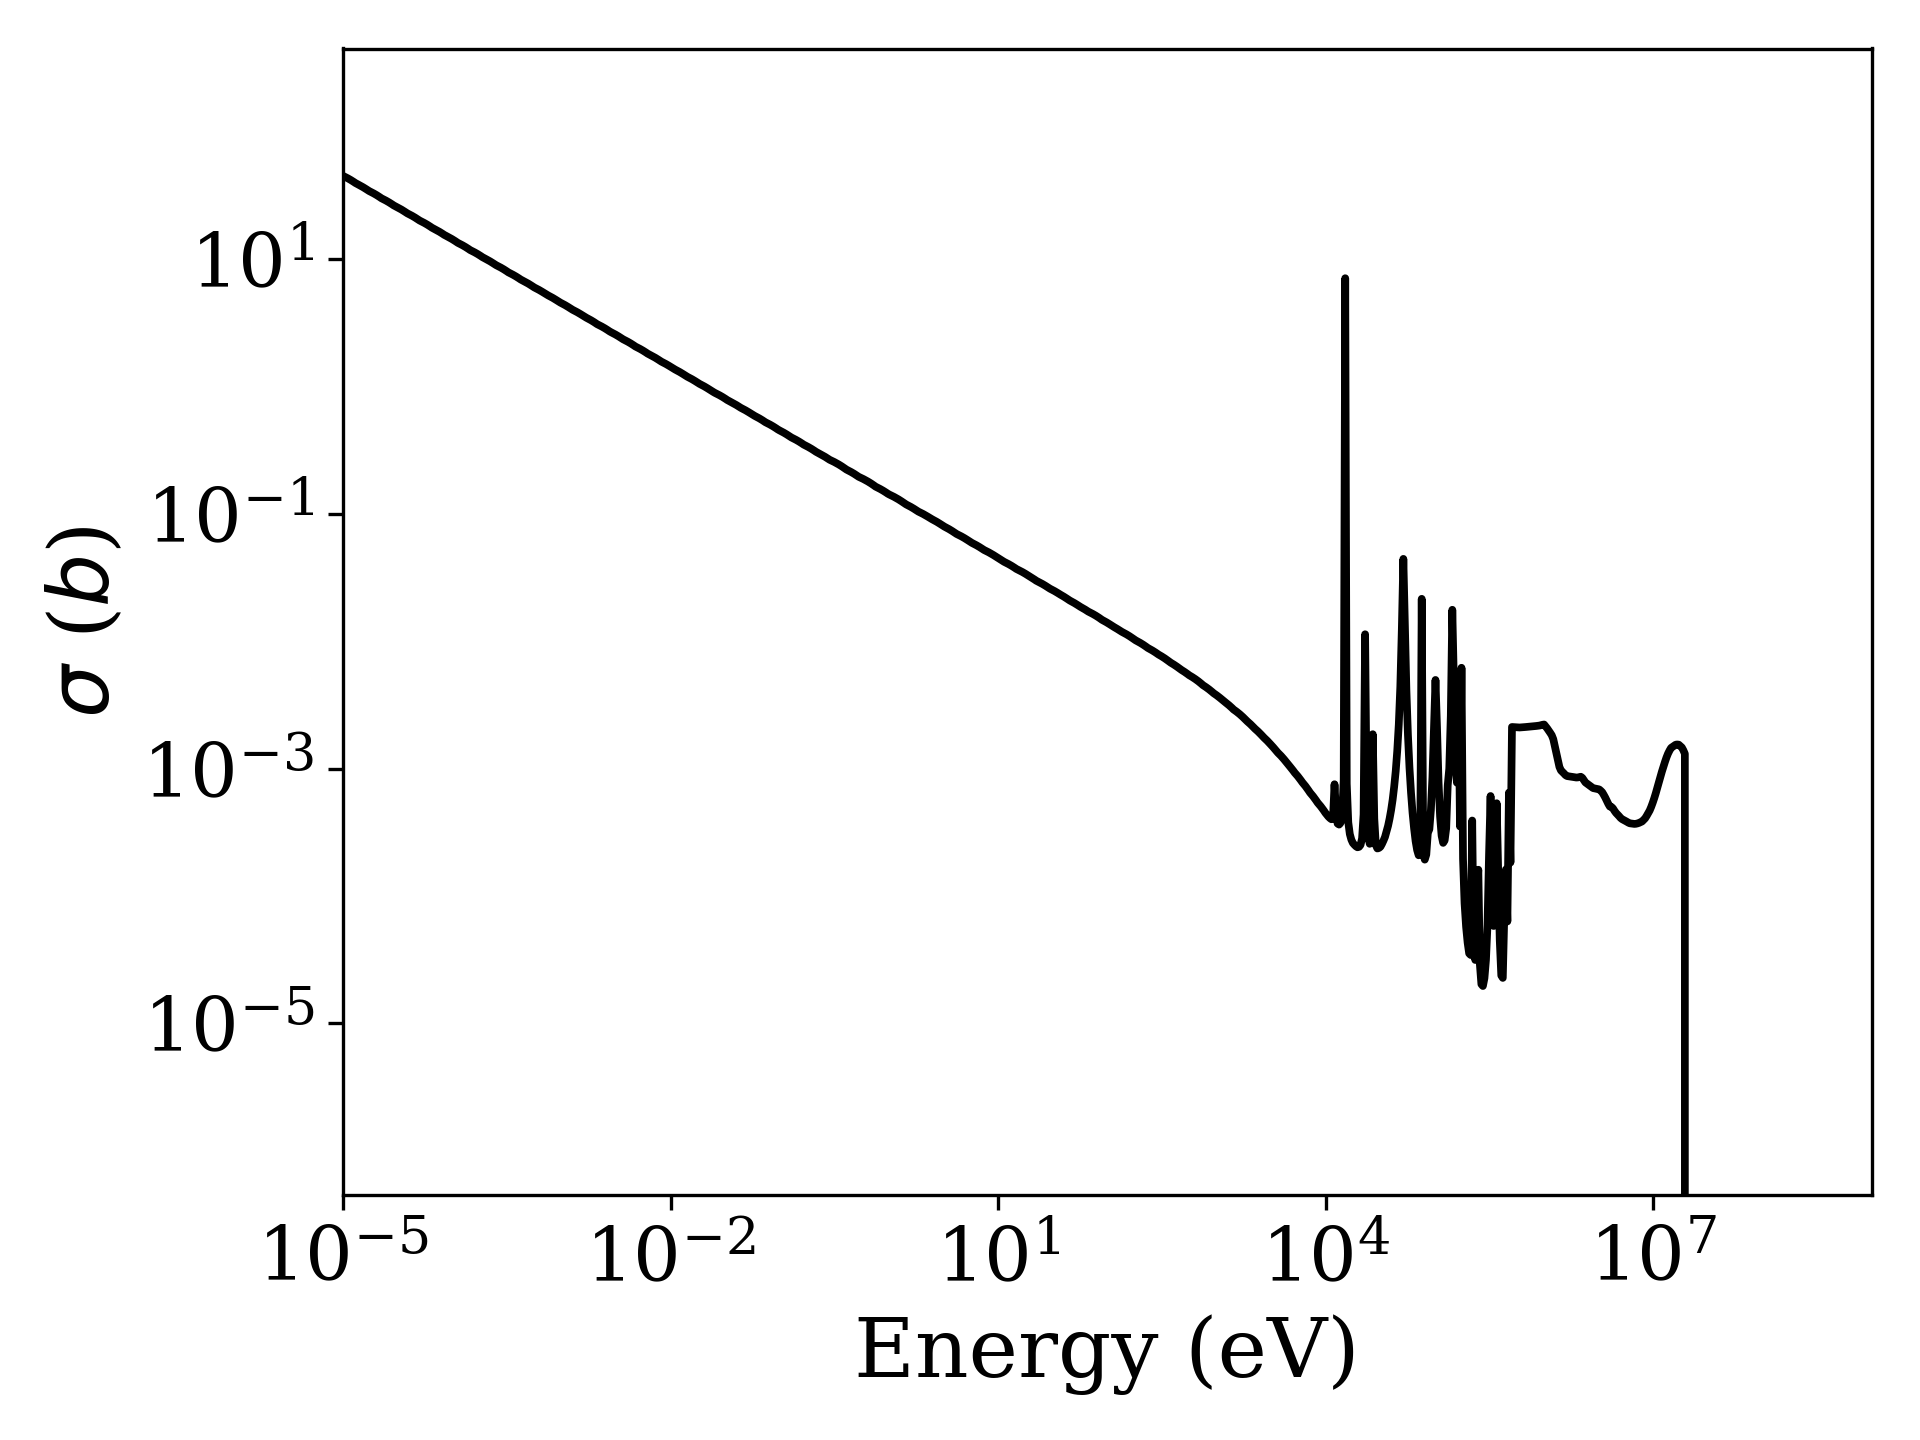
\includegraphics[width=.8\textwidth]{plot/Ca-44(n,gamma)Ca-45} 

  \caption{A subfigure}
  \label{fig:sub2}
\end{subfigure}
\caption{A figure with two subfigures}
\label{fig:test}
\end{figure}

\begin{table*}[h]
\centering
\begin{tabular}{ |c|c|c|c|c|c|c| }
 \hline
 Reaction & T$_{1/2}$ & ROI (eV) & Important Gammas (keV) \\
 \hline 
 $^{44}$Ca(n,$\gamma$)$^{45}$Ca & 165.0 d & 6.68e-03, 6.38e-01 & 12.47(3e-08) \\ 
\hline
\end{tabular}
\end{table*}
